

%!TEX root = /Users/kevin/SkyDrive/KTH Work/LaTeX Reports/HW4-High Resolution shock-capturing methods/HW4_High_Resolution_shock_capturing_methods.tex
\section{First order Roe scheme} 
\subsection{Roe tests with flat bottom} % (fold)
\label{sub:roe_tests_with_flat_bottom}

% subsection roe_tests_with_flat_bottom (end)
% (fold)
\label{sec:first_order_roe_scheme} 
\begin{enumerate}
	\item 
	\begin{enumerate}
		\item Explain how to choose m(x,0), to make a single pulse (not two!) based on the linearized problem. 
		
		You can make it a single pulse by giving the wave an initial speed proportional to its height in one direction. Since $m=hv$, we can set m to $hc$, where the characteristic speed is $c=\sqrt{gH}$, and $H=0$ since we want a linearized approximation.
		
		\item Use this initial data and run the Roe solver with n=80, 160, 320 and the CFL number as large as possible without instability, until the wave has been fully reflected at L. Plot the wave shapes. 
		
		Figure~\ref{fig:Figure21} shows the plots using different N values.  The N value seemed to affect the sharpness of the front edge of the wave. As N increased, the sharpness increased.  
		\begin{figure}
			[htbp] \centering 
			\subfigure[$N=80$ \label{fig:Figures_plot2p1_n_is_80}]{ 
			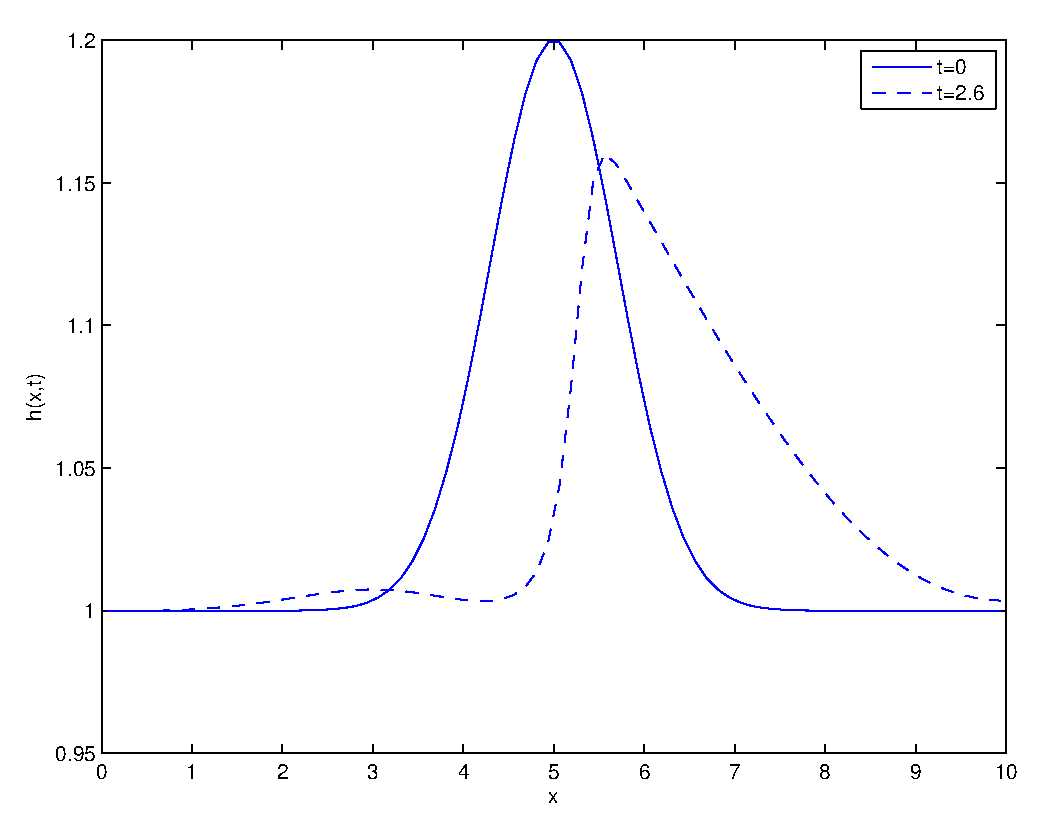
\includegraphics[width=\hpage]{Figures/plot2p1_n_is_80.eps}} \hspace{5pt} 
			\subfigure[$N=160$ \label{fig:Figures_plot2p1_n_is_80}]{ 
			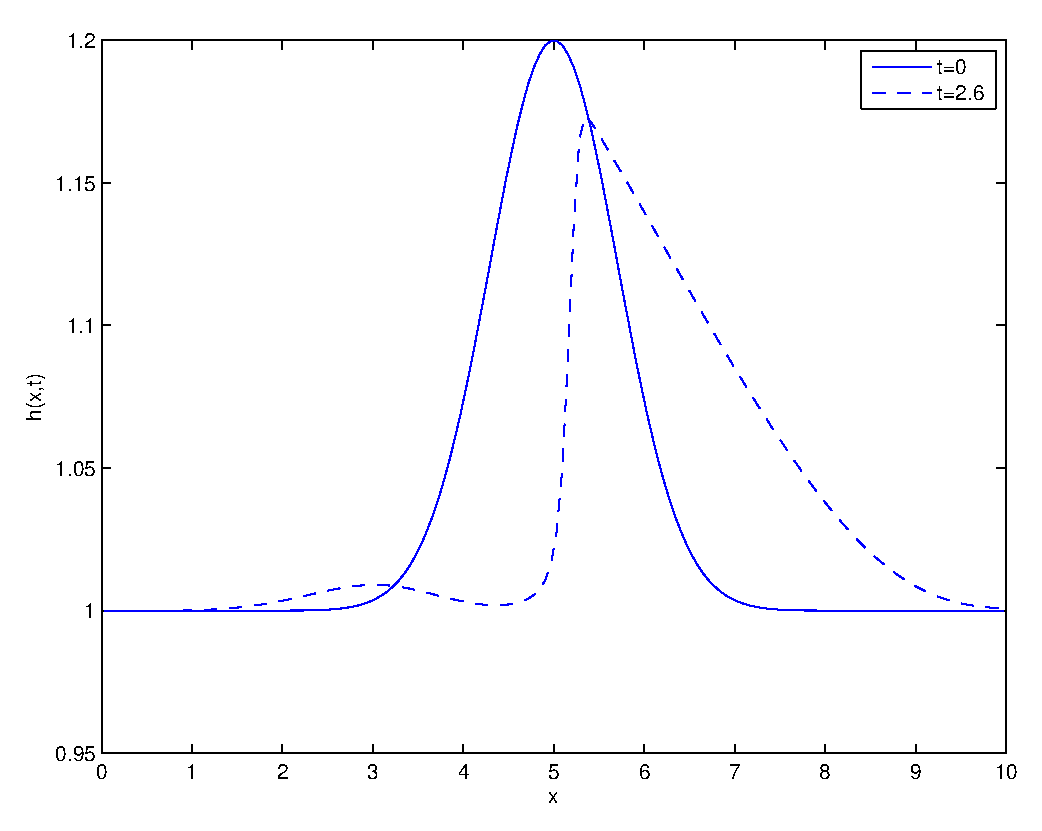
\includegraphics[width=\hpage]{Figures/plot2p1_n_is_160.eps}} \label{fig:Figures_plot2p1_n_is_160}
			\subfigure[$N=320$ \label{fig:Figures_plot2p1_n_is_320}]{
			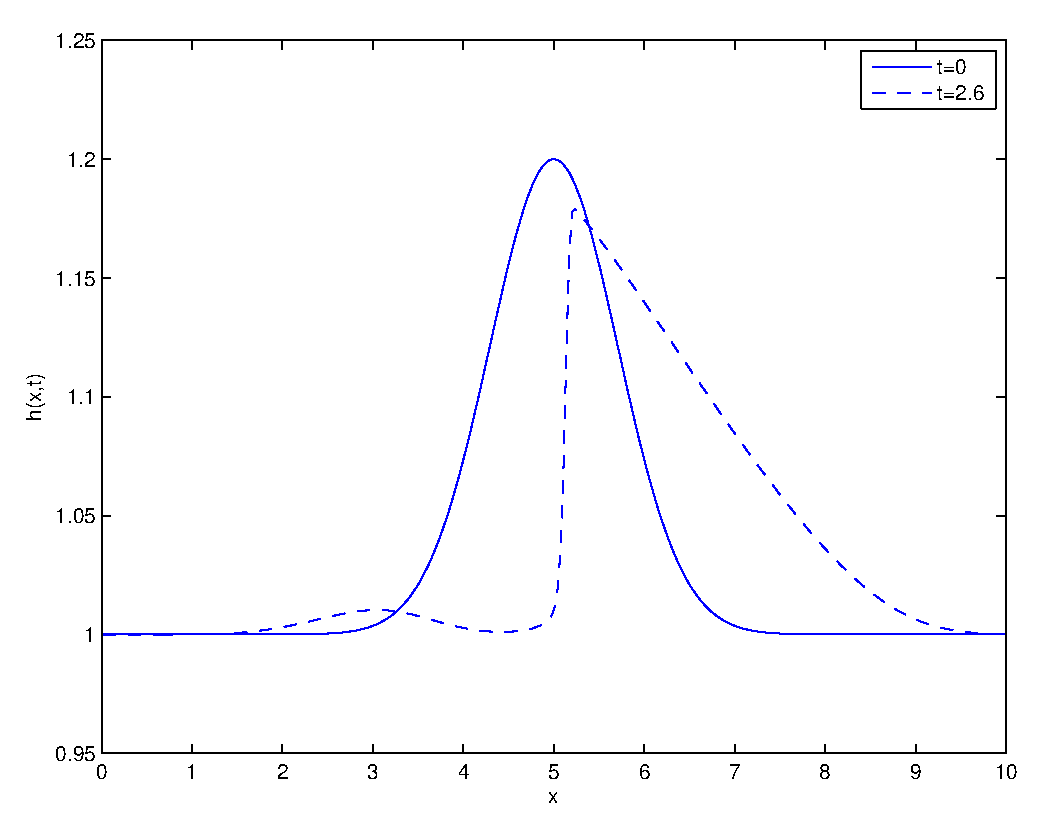
\includegraphics[width=\hpage]{Figures/plot2p1_n_is_320.eps}}
			\caption{These are the plots with different N values.  The CFL condition was set to 80\% of the value that would be ideal for a linear problem. The wave edges get sharper when $N$ is increased} 
			\label{fig:Figure21}
		\end{figure}
		
		\item Compare with solutions obtained using your Lax-Friedrichs solver from HW2. 
		
		The solution obtained here looks very similar to the Lax-Friedrichs solver from HW2 as the shape of the wave forms a sharp edge and looks like a triangle instead of a Gaussian.  This solution isn't stable at the CFL condition and we must make the time step a little smaller.  The Lax-Friedrich solution was also not stable at the CFL condition, but I was forced to decrease the time step by a much larger amount in order to see stability for a few seconds.
		\item Comment about order of accuracy, dissipation and dispersion. 
		The dissipation around the edges decreases as we increase the value of N.  But increasing the value of N too much will only cause instabilities.
		
		\item Then try also a higher pulse, say a = 2H. Comment on how well the single pulse initial data works. 
		
		A pulse with $a>1/5 H$ gives unstable results using a time step of 80\% of the CFL condition, so I had to reduce it to 40\% in order to get the results shown in Figure~\ref{fig:Figure21d}.  This figure is different from Figure~\ref{fig:Figure21} in that the height of the left moving pulse isn't as negligible as it once was.  The overlap of the smaller wave is much more noticeable when $a$ is large compared to H. 
		
		\begin{figure}
			[htbp] \centering 
			\subfigure[$N=80$ \label{fig:Figures_plot2p1_n_is_80_a_2}]{ 
			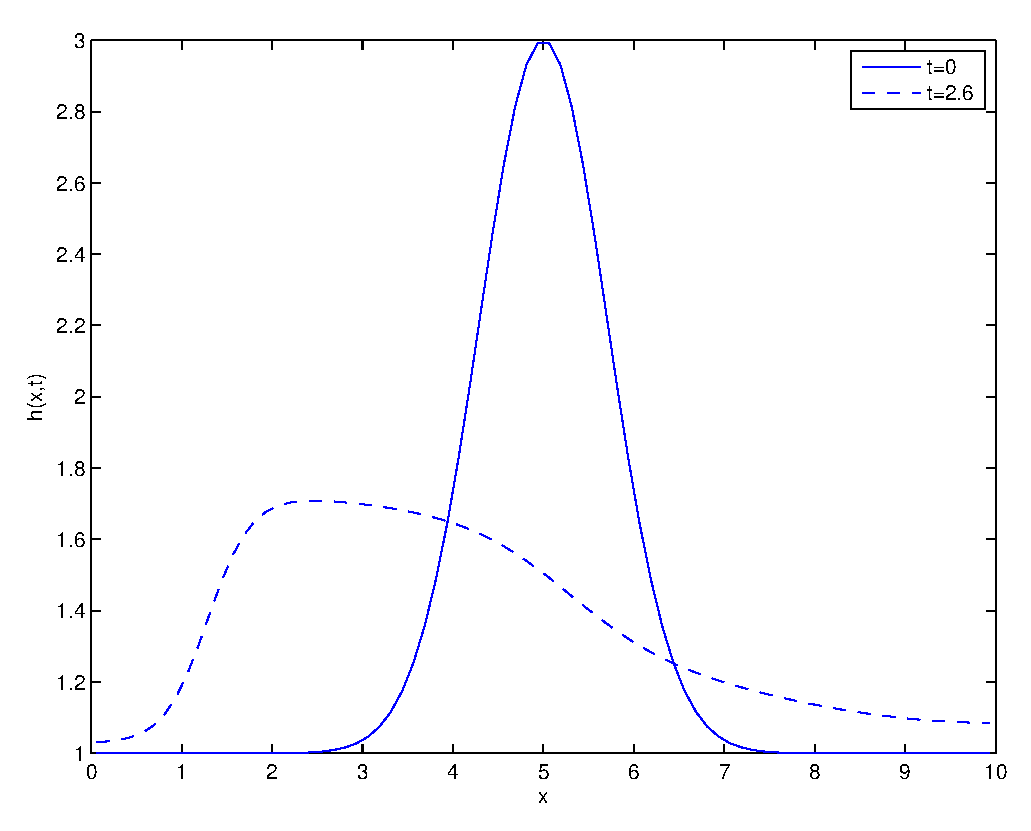
\includegraphics[width=\hpage]{Figures/plot2p1_n_is_80_a_2.eps}} \hspace{5pt} 
			\subfigure[$N=160$ \label{fig:Figures_plot2p1_n_is_80_a_2}]{ 
			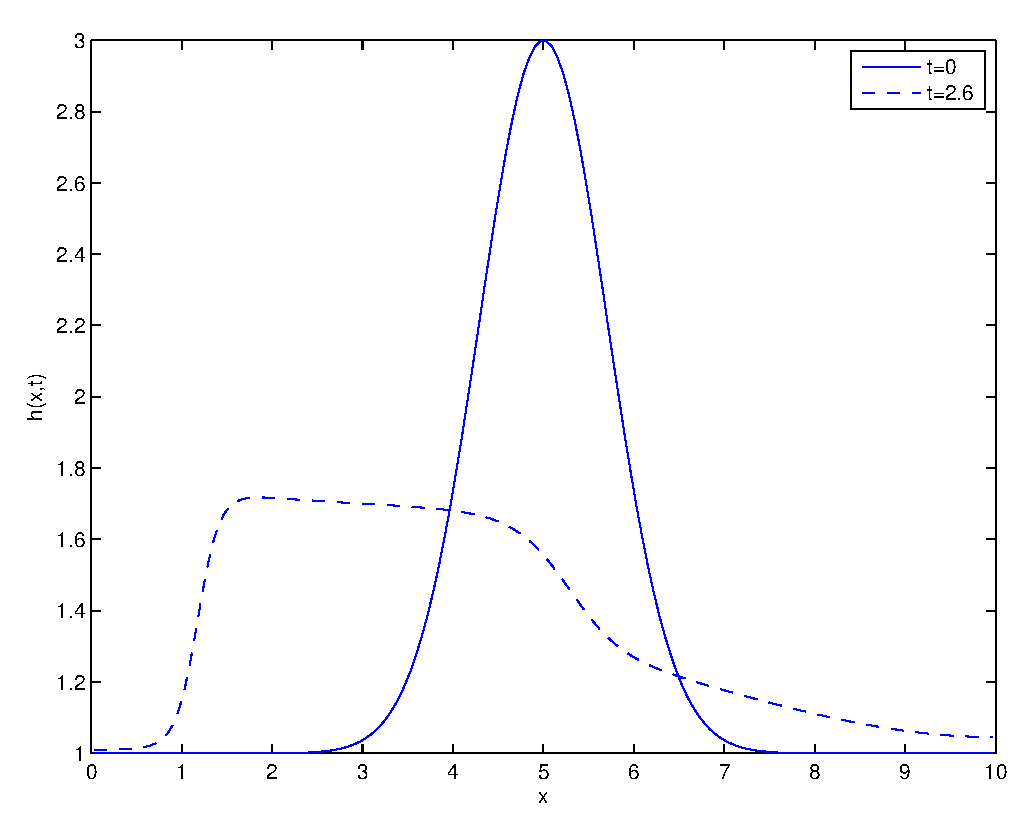
\includegraphics[width=\hpage]{Figures/plot2p1_n_is_160_a_2.eps}} \label{fig:Figures_plot2p1_n_is_160_a_2}
			\subfigure[$N=320$ \label{fig:Figures_plot2p1_n_is_320_a_2}]{
			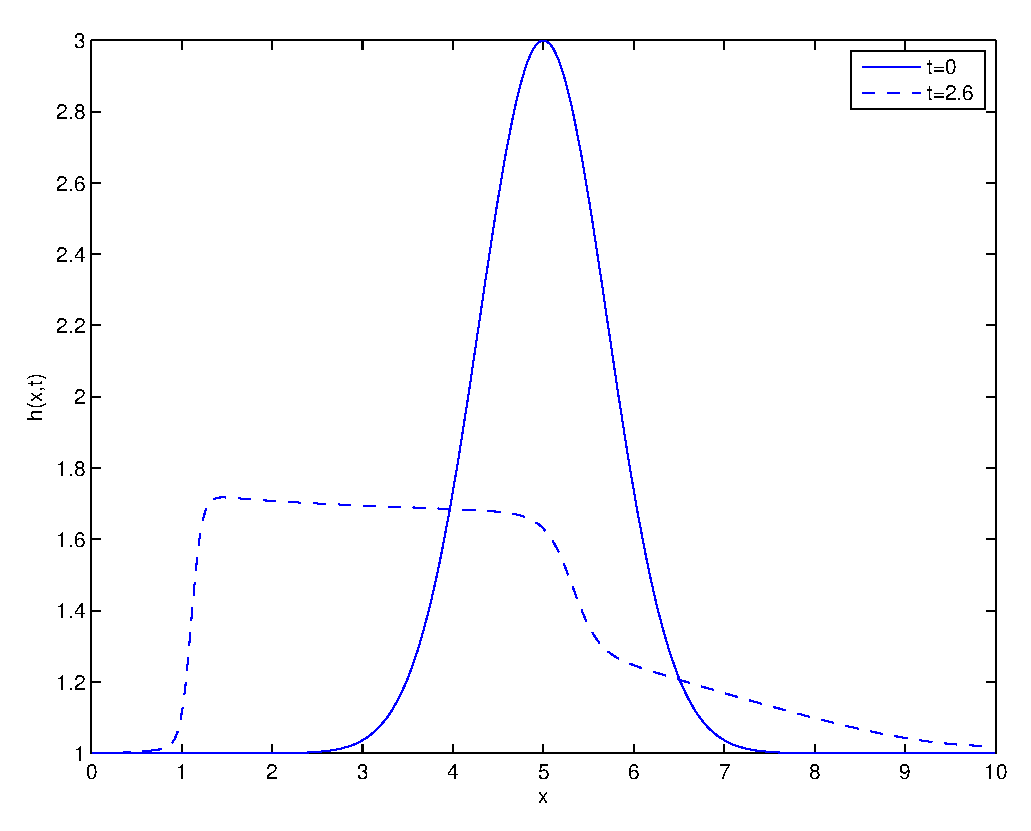
\includegraphics[width=\hpage]{Figures/plot2p1_n_is_320_a_2.eps}}
			\caption{These are the plots with different N values.  The CFL condition was set to 40\% of the value that would be ideal for a linear problem. The wave edges get sharper when $N$ is increased, but changing the value of $a$ has also changed the characteristic speed and shape of the wave after it recombines with its small wave that moves leftward.} 
			\label{fig:Figure21d}
		\end{figure}
		
	\end{enumerate}
\end{enumerate}

% section first_order_roe_scheme (end)
